\chapter{Conclusion}
\label{ch:conclusion}
\epigraph{\itshape``Of everything that man erects and builds in his urge for living, nothing is in my eyes better and more valuable than bridges. They are more important than houses, more sacred than shrines. Belonging to everyone and being equal to everyone, useful, always built with a sense, on the spot where most human needs are crossing, they are more durable than other buildings and they do not serve for anything secret or bad."}{--- \textup{Ivo Andri\' c}}

\section{Introduction}
\hspace{10pt} The following sections serve as a brief introduction to the ongoing work focused on combining the efforts from all analyses searching for the invisible final state of the Higgs boson\footnote{Summarising the Run 2 phase of operation. The previous combination summarising early Run 2 (2015 and 2016) and Run 1 is detailed in Ref.~\cite{paper:HIG_17_023}.}. %This result presents a first look into the final (leagacy) result of the Run 2 phase for these processes. The first section will focus on the description of a common data processing and analysis framework, developed with the combination effort in mind. The main benefit of such approach comes from the possibility to use same treatment of uncertainties for shared sources, making the combination effort much more robust. Another important benefit arising form this approach is the out of the box orthogonality, which will be described in the following sections. Following the description of each of the categories (covering the non VBF strategies brefly mentioned in Chapter~[R]), this part of the discussion is going to be concluded with a set of preliminary combination results.
Finally, in order to have a complete narrative when describing the H$\rightarrow$inv studies, there is one more era that needs covering - the future. The main idea and the previously obtained results have been the focus of Part 1 of this thesis, while the present has been represented with all the Run 2 efforts covered in Parts 2 and 3. In order to come to a proper conclusion, this chapter is going to contain a discussion about studies of future prospects for this channel with respect to the later phases of the LHC and corresponding upgrades of the CMS detector.

\section{The grand combination}

\hspace{10pt} The VBF production mode represents the leading channel in terms of sensitivity towards the invisible final state of the Higgs boson. As introduced in Chapter~\ref{ch:Higgs_LHC_DM}, the other production modes have been explored in order to have the best possible coverage of interesting phase space. The approach taken early on in the development of these analyses for the 2017-18 data taking period was to create exclusive channels which will be sorted by the importance towards the final state. This has led to the VBF taking the prime spot within the event processing cycle, and if an event didn't satisfy the conditions of the VBF channel it would begin its journey towards the non-VBF clusters of categories. 

\hspace{10pt} The non-VBF categorisation follows a similar strategy to the older approaches, but modifies the traditional channel ordering based on the production mode in question (namely ggH, VH, and ttH) in favour of subcategories whose expected sensitivity is estimated through an optimisation technique based around the S/$\sqrt{\text{B}}$ criteria\footnote{The S and B parameters denote the overall signal and total background yields, where the expected sensitivity term connects to the fact that this is an estimation relying purely on simulated samples.}. Having designed the event categorisation in such an orthogonal way there is one more important aspect which, if properly approached, would make for a smooth combination. This aspect is seen in the way these categories share the treatment of uncertainties. Sharing of as many input parameters which form these analyses allows for a by design level of consistency usually seen only after a hard work of connecting different parameters and inputs through the scan of inputs from different analysis teams using different software packages. This is where the more technical aspect comes to light - nothing is stopping the analysers from taking this combined analysis strategy and implementing it in a novel analysis framework. One larger effort could also help overcome general problems affecting HEP analyses as a whole (large time intervals needed when processing datasets, different output files used by various teams, rigid software having a steep learning curve, etc).



%\hspace{10pt} The culmination of measurements from both the VBF and non VBF types of analyses is going to be summarised. This section will conclude with the first look into the overall sensitivity being presented. In order to do be able to efficiently present the overarching idea, the first section is going to present an overview of the whole approach. Previously these studies were all parts of separate studies that were optimised in the end for the H$\rightarrow$inv combination (as mentioned in Chapter~[R]). This approach allowed for out of the box sharing object corrections, sources of uncertainties and immediate phase space orthogonality through the optimisation specifically tailored for the H$\rightarrow$inv decay mode. The following pages are going to summarise the first result born from this effort.


\hspace{10pt} This is where the Faster Analysis Software Taskforce (FAST)~\cite{twiki:fast} framework comes into focus. It represents the main data processing software used for the purposes of these studies. It is based on standard python libraries which allow for the usage of dataframes, array techniques and easy to read/write configuration files\footnote{The inclusion of different array techniques allows for the removal of an event loop, instead relying on a "chunk" of data being loaded and operated on at the time. This overcomes the main issue which comes in mind of many when choosing more traditional C++ based processing tools - processing speed}. This approach  bridges a connection between industry standards and science. One of the benefits arising from this sort of data processing is the lightweight output in the form of standard dataframe formats and its support for modular designs. 

\hspace{10pt} This embrace of modular design philosophy is especially important when it comes to previously discussed combination efforts as the main analysis framework was built to explore all the benefits of this data processing approach. All channels would be dependent on a set of core software modules creating base analysis object collections, while all other specifics can be implemented through a set of custom modules, which can simply be added in the chain without much effort. Finally, this approach brings the usage of configuration files which are based on the easy to read data-serialisation language - YAML~\cite{twiki:yaml}. They are basically used to summarise which modules are deployed in the analysis, how the important regions are defined and what output is needed. This reduces the debugging time significantly by keeping all core analysis inputs defined in a single location.

%These lines were supposed to introduce more details of the aforementioned combination effort. Unfortunately due to the fact that timelines of this thesis and the combination effort weren't completely aligned, this is as much details as the author is allowed to go into at this stage.
\hspace{10pt} The previously described VBF H$\rightarrow$inv study represents the first step in the combined analysis. The sensitivity given by the VBF analysis (and its comparison with other channels presented in Chapter~\ref{ch:Higgs_LHC_DM}) can serve as a good figure of merit regarding what can be expected from other channels, which due to a more detailed categorisation are expected to yield a better result compared to what would be achieved by keeping the old strategy. These non-VBF studies are currently in progress and are the main focus of Ref.~\cite{thesis:esh}, where this approach is presented in much more detail.



%\subsection{Overview}
%\hspace{10pt} With the VBF analysis being the main focus of previous chapters, this section is going to move the spotlight closer towards the approach taken with the non VBF analyses. As already introduced in Section~\ref{ch:an_strategy}, the non VBF analyses represent a collection of studies (in further text categories) revolving around hadronic production modes of the Higgs boson other than the VBF. Figure~\ref{fig:chip} shows a graphical representation of the overall categorisation process an event goes through in the combine analysis. 
%\begin{figure}[htbp]
%  \centering
%    \includegraphics[width=0.8\textwidth]{example-image-a}
%  \caption{Diagram of the event categorisation used for the combined H$\rightarrow$inv study~\cite{note:AN_18_299,note:AN_19_257}}
%  \label{fig:chip}
%\end{figure}



\section{A look into the future}
\hspace{10pt} Due to its strong dependence on forward jets and $E_{T,miss}$, the VBF H$\rightarrow$inv analysis represents a good way to test the potential sensitivity gains and modified reconstruction algorithms arising with upgrades of the CMS detector for various operational conditions of the LHC which are expected to be reached in the future (such as the HL-LHC phase~\cite{paper:hl-lhc}). This is the purpose of studies published in Ref.~\cite{yellow_report} where, on the altruistic side, the performance of reconstruction algorithms designed to incorporate upcoming upgrades (such as the HGCal upgrade~\cite{paper:hgcal}) is tested. On the more analysis oriented side, they can be used to test how the expected sensitivity of the current approach scales with the size of the dataset and to see if these strategies are still viable for upcoming phases.

\hspace{10pt} A simulation study of H$\rightarrow$inv analysis prospects was performed for three different values of total integrated luminosity: $L=$~300, 1000 and 3000~$\text{fb}^{-1}$. The simulation of detector effects was performed using the Delphes software package~\cite{paper:delphes} (which mimics the upgraded state, Phase 2, of the CMS experiment\footnote{This includes the increase in the number of pile-up interactions to 200 and the expected increase in the operational energy to 14 TeV.}). The analysis strategy approached here was to use the main MTR analysis category (defined similarly to what is described in Chapter~\ref{ch:an_strategy}). The assumption made at the beginning was that the $E_{T,miss}$ triggers would perform in such a rate-controlled way that they would allow for even lower $E_{T,miss}$ thresholds than what was used during the Run 2 phase. Figure~\ref{fig:yr_distributions} shows the background composition in the signal region for two main variables of interest: the $E_{T,miss}$ and the dijet mass.


\begin{figure}[htbp]
  \centering
    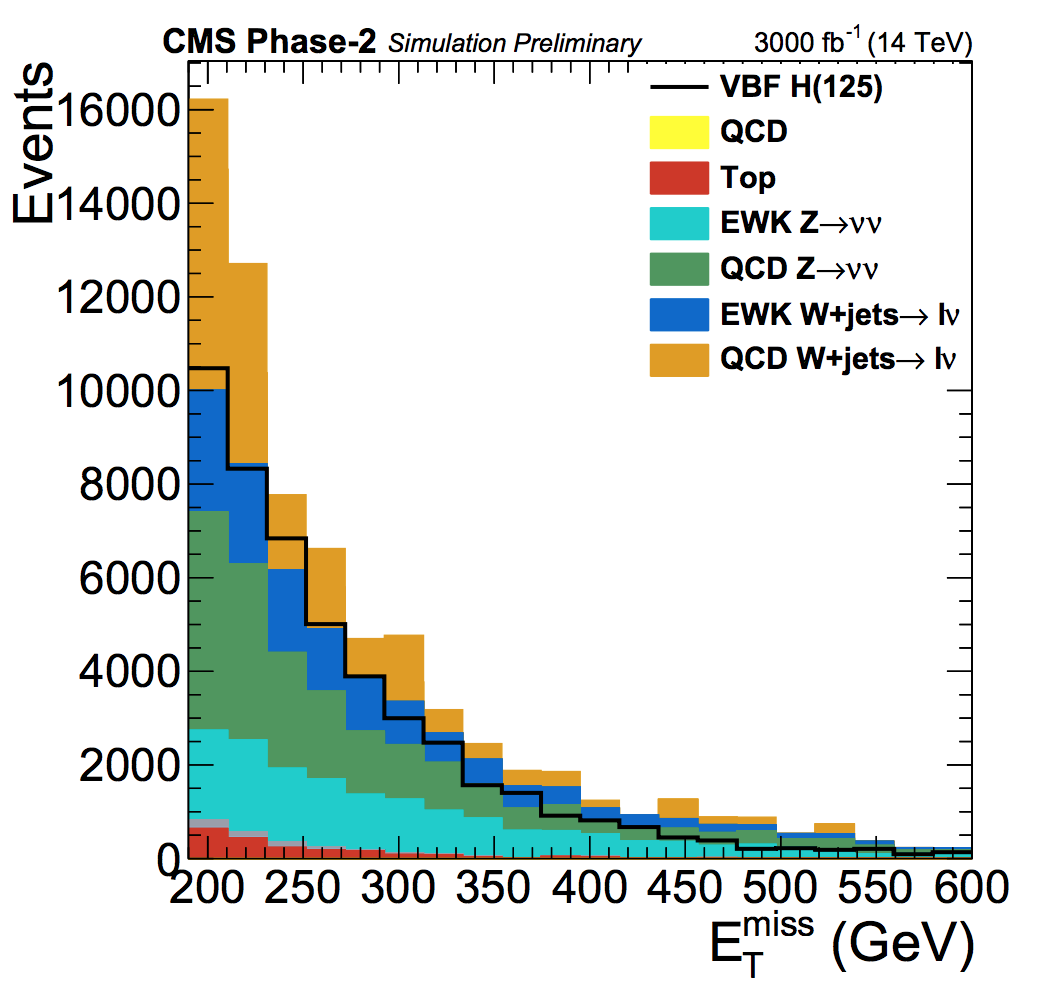
\includegraphics[width=0.49 \textwidth]{Conclusion/YR_MET.png}
    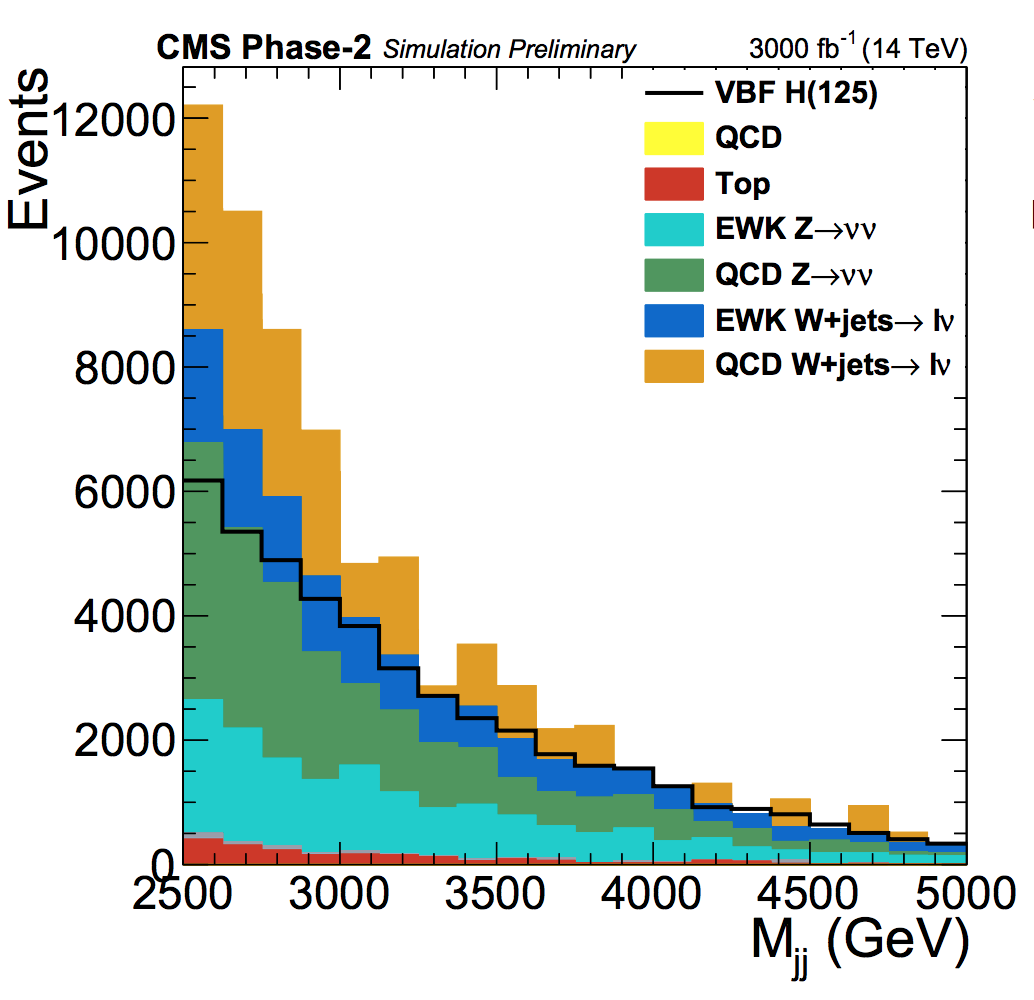
\includegraphics[width=0.49\textwidth]{Conclusion/YR_mjj.png}

  \caption{Composition of background processes overlayed with the signal simulation in the SR for $E_{T,miss}$ (left) and $m_{jj}$ (right)~\cite{yellow_report}.}
  \label{fig:yr_distributions}
\end{figure}
\hspace{10pt} An optimisation was performed varying the ranges of these two variables with the purpose of obtaining the best constraint on the invisible final state. The resulting 95\% CL upper limits expressed as a function the the respective $E_{T,miss}$ thresholds are shown in Figure~\ref{fig:yr_limits} for three scenarios of total integrated luminosity\footnote{For a $m_{jj}$ threshold which resulted from optimisation of each of these scenarios. The treatment of uncertainties follows the Run 2 approach albeit with small differences when it comes to better expected performance of the CMS experiment (the same can be said for the definitions of object collections) and is discussed in more details in Ref.~\cite{yellow_report}.}. By focusing on the minima for each of three scenarios it can be seen that the expected limit value does not decrease significantly simply due to an increase in total integrated luminosity. This indicates that, besides a constant improvement of the theoretical uncertainty treatment, this analysis needs to develop a better approach (akin to the one taken in 2017-18 period with a dedicated VBF trigger) in order to further increase the sensitivity towards the invisible final state. The best reported constrain on the B(H$\rightarrow$inv) is obtained to be 3.8~\% (expected for the scenario with $L =$~3000~$\text{fb}^{-1}$).

\begin{figure}[htbp]
  \centering
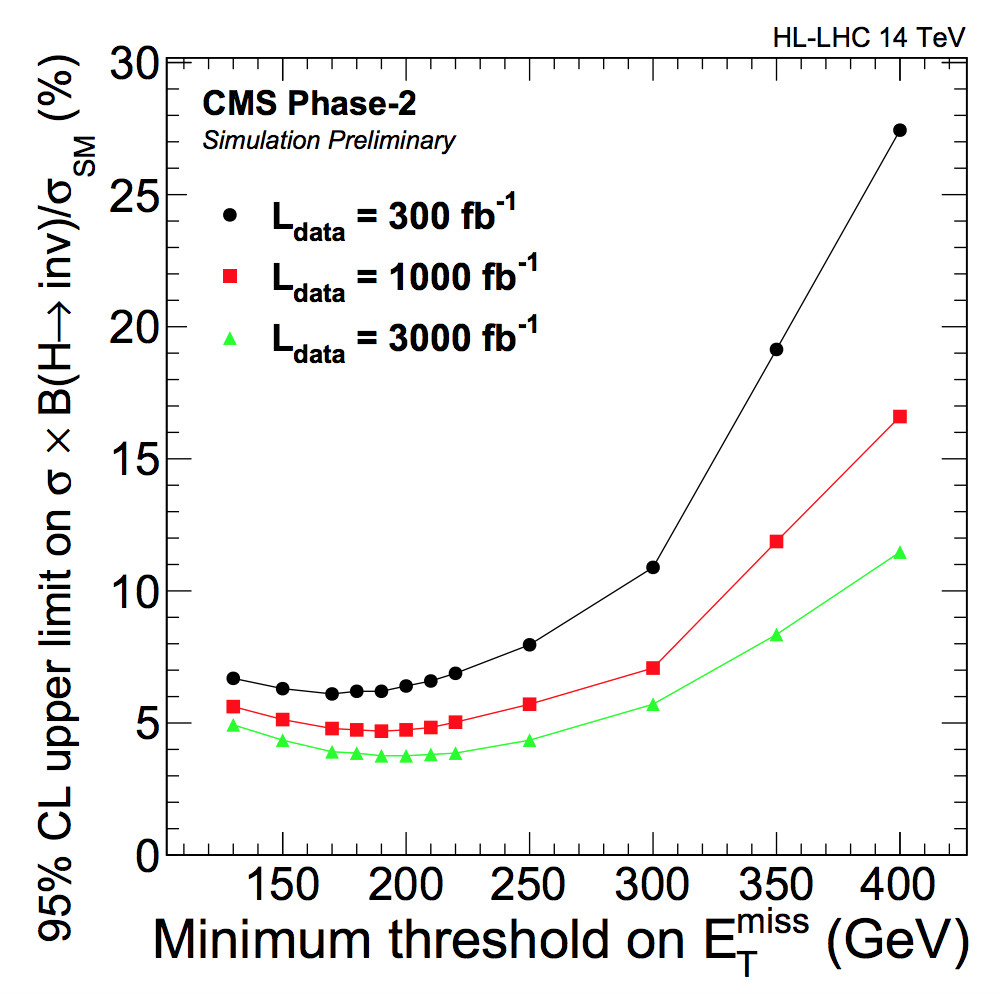
\includegraphics[width=0.49 \textwidth]{Conclusion/YR_limit1.png}
    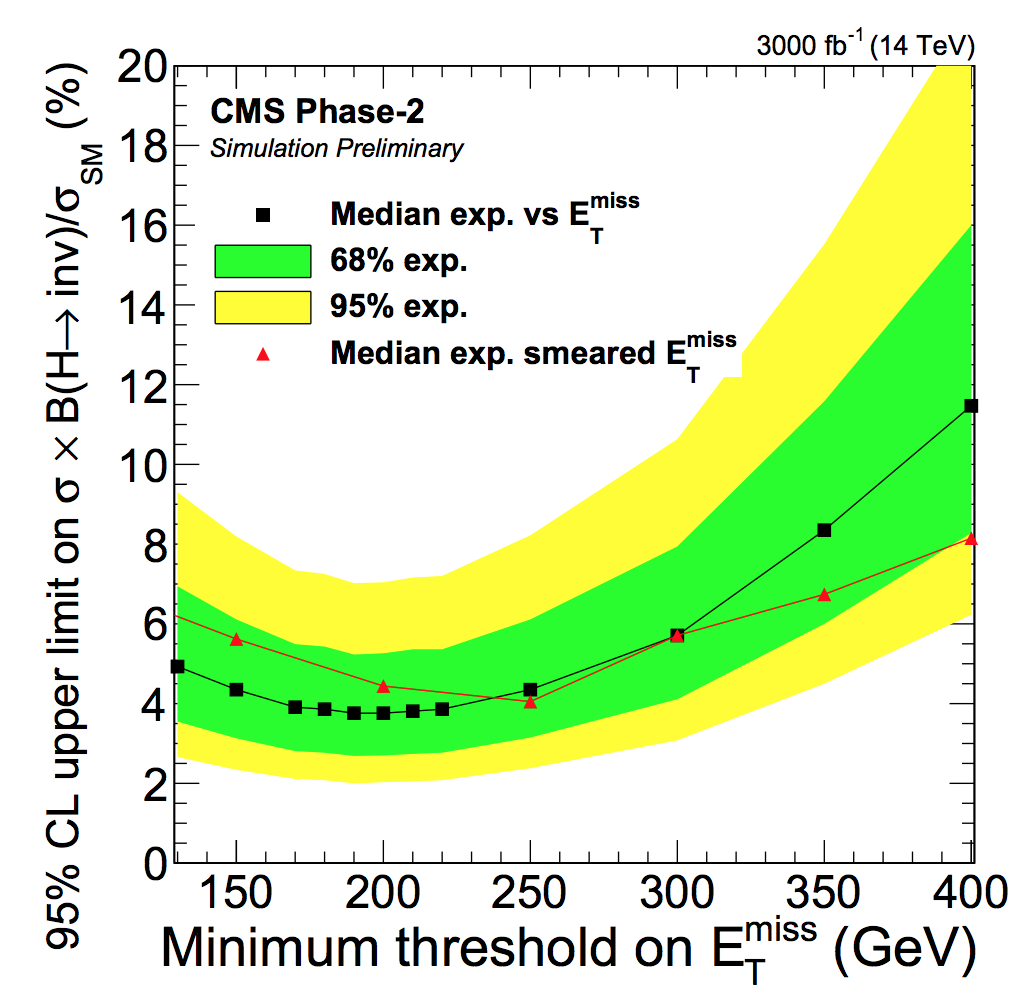
\includegraphics[width=0.49\textwidth]{Conclusion/YR_limit2.png}

  \caption{Estimation of the 95\% CL upper limits presented for different values of the $E_{T,miss}$ threshold for three different scenarios based on the values of total integrate luminosities (left), and the detailed look at the behaviour of the upper limit bands for the most sensitive scenario of $L=$~3000~$fb^{-1}$ (right)~\cite{yellow_report}.}
  \label{fig:yr_limits}
\end{figure}

\hspace{10pt} A similar simulation study has been performed by the ATLAS collaboration, this time targeting the the second most sensitive channel - the VH production mode. Their projection gives an 95\% CL upper limit value of 8\%, which can be further combined with the previously presented study. Making one more assumption, that both experiments are expected to perform similarly in all channels, the final combination provides a total projected constrain on the B(H$\rightarrow$inv)~$\leq$~ 2.5\%\footnote{When assigning the same VBF result to the ATLAS measurement and vice versa.} for the HL-LHC phase of operation.
\section{Final words}
\hspace{10pt} A search for the invisible decays of Higgs bosons was presented. Specific triggers have been shown following the entire study process from the trigger design until the final result. Discussion of the results has been presented in three eras: past, present and future. The overview of the past era introduced the method and corresponding results in a chronological manner, showing the motives and ideas behind these studies and their realisation. The present was used as an example of how these studies can mature, take advantage of the technical advancements of the detection process and showed a first look at the full Run 2 result. A peak behind the curtain showed that a more analysis focused approach taken with the Run 2 VBF trigger is going to be of even greater importance  for the next phases, as it will be crucial to have trigger strategies that will efficiently target interesting topologies.

\hspace{10pt} The upcoming period leaves a lot of opportunities for young researchers to start their journey. A prospect of being able to build the entire analysis process from the first, trigger level until and follow it trough until the end result is, from the author's point of view, the best possible reward one can get from PhD studies. The amount of experience gained and the ability to appreciate how every small piece forms the bigger picture is an gift very few endeavours provide as a result.

\hspace{10pt} The final result of this thesis summarises that there was no observed deviation from the SM with respect to the process of interest. An 95\% CL upper limit has been set on the branching ratio of the VBF H$\rightarrow$ inv decay and it currently stands at XX (XX) expected (observed) value for the 2017-18 data taking period, while the combination effort with the study focusing on the 2016 era yields a Br(VBF H$\rightarrow$inv)~$=$~XX (XX). These results present a preliminary status, which is expected to be improved on when the final result is published in the near future.